%%%%%%%%%%%%%%%%%%%% author.tex %%%%%%%%%%%%%%%%%%%%%%%%%%%%%%%%%%%
%
% sample root file for your "contribution" to a contributed volume
%
% Use this file as a template for your own input.
%
%%%%%%%%%%%%%%%% Springer %%%%%%%%%%%%%%%%%%%%%%%%%%%%%%%%%%


% RECOMMENDED %%%%%%%%%%%%%%%%%%%%%%%%%%%%%%%%%%%%%%%%%%%%%%%%%%%
\documentclass[graybox]{svmult}

% choose options for [] as required from the list
% in the Reference Guide

\usepackage{mathptmx}       % selects Times Roman as basic font
\usepackage{helvet}         % selects Helvetica as sans-serif font
\usepackage{courier}        % selects Courier as typewriter font
\usepackage{type1cm}        % activate if the above 3 fonts are
                            % not available on your system
%
\usepackage{makeidx}         % allows index generation
\usepackage{url}             % links
\usepackage{graphicx}        % standard LaTeX graphics tool
                             % when including figure files
\usepackage{multicol}        % used for the two-column index
\usepackage[bottom]{footmisc}% places footnotes at page bottom

\usepackage{algorithm}
\usepackage[noend]{algpseudocode}

% see the list of further useful packages
% in the Reference Guide

\makeindex             % used for the subject index
                       % please use the style svind.ist with
                       % your makeindex program

%%%%%%%%%%%%%%%%%%%%%%%%%%%%%%%%%%%%%%%%%%%%%%%%%%%%%%%%%%%%%%%%%%%%%%%%%%%%%%%%%%%%%%%%%

\begin{document}

\title*{Accelerated Load Balancing of Unstructured Meshes}
% Use \titlerunning{Short Title} for an abbreviated version of
% your contribution title if the original one is too long
\author{
Gerrett Diamond,
Lucas Davis,
and Cameron W. Smith
}
\institute{
  Gerrett Diamond \email{diamog@rpi.edu}
  \and Lucas Davis \email{davisl3@rpi.edu}
  \and Cameron W. Smith \email{smithc11@rpi.edu}
  \at Rensselaer Polytechnic Institute, Troy, NY 
}
\authorrunning{G.Diamond et al.}

\maketitle

\abstract{
Unstructured mesh applications running on large, parallel, distributed memory
systems require the computational work related to mesh entities to be evenly
distributed across processes in order to achieve maximal performance.
To efficiently balance meshes on systems with accelerators the balancing
procedure must utilize the accelerator.
This work presents algorithms and speedup results using OpenCL and Kokkos to
accelerate critical portions of the EnGPar diffusive load balancer.
}

\section{Introduction} \label{sec:intro}

%\begin{itemize}
%  \item briefly motivate dynamic load balancing
%  \item quantify how GPUs are providing the majority of computing performance (\# of systems with GPUs in top 10 systems of top500, graph500, HPCG)
%  \item end with a sentence that says what engpar does (diffusion) and how we are
%extending it to run on GPUs
%\end{itemize}

While common partitioning techniques such as multilevel or geometric methods are
good for creating an initial distribution of load, those techniques are not as
applicable  to simulations where the mesh and load changes.
These evolving simulations require dynamic load balancing techniques that are
quick to improve the partition.
Diffusive load balancing methods allow quick partition refinement for the
relatively small changes to imbalance that are seen in adaptive mesh
simulations.
EnGPar's diffusive balancer has been shown to quickly produce high quality
partitions at up to 512Ki processes~\cite{engparSC17}.

\section{EnGPar Dynamic Load Balancing} \label{sec:engpar}

%\begin{itemize}
%  \item multi-graph, high-level diffusion algorithm (targeting, selection, migration)
%  \item indicate that we will accelerate selection via BFS for distance computation and coloring for cavity selection
%\end{itemize}

EnGPar is a partition improvement tool that utilizes a multi-hypergraph,
called the N-graph, to describe the portions of the mesh that require load balancing.
The N-graph consists of vertices which represent the primary dimension entities of the
mesh. The vertices are connected by hyperedges created from the secondary dimensions of
the mesh that require load balancing.

EnGPar's diffusive algorithm is an iterative local refinement strategy.
In each iteration the target criteria is improved until the imbalance is under a
given tolerance or the imbalance cannot be improved further.
Each iteration consists of three steps: targeting, selection, and migration.
The targeting step gathers metrics on the part and its neighbors
in order to determine which neighboring parts to send weight to and how much
weight to send.
The selection step is where graph vertices on the boundary are chosen to be sent
to neighboring parts in order to satisfy the weights determined by the targeting
phase.
Finally, the migration step sends the graph entities that were selected to the
destination parts and the graph is reconstructed.

In this work, we target accelerating distance computation and cavity selection.
These two procedures consume up to 50\% of the total execution time and are well
suited to acceleration as they do not require inter-process communications~\cite{engparSC17}.

Distance computation is performed during selection by ordering hyperedges on the
boundary based on their distance from the center of the part from furthest to
closest.
EnGPar computes this distance with two breadth first traversals of the graph.
The first traversal starts at the part boundary and works its way in while
marking the depth of visited hyperedges.
The second traversal starts from a hyperedge with the largest depth and works
its way out to the boundary while marking the distance from the starting point.

Cavity selection determines if a cavity, defined as a hyperedge and the vertices
that are connected by it, on the part boundary should be sent to one of the
neighboring parts.
A cavity is selected for migration if (1) the part that the hyperedge is shared
with is a target part, (2) the target part has not been sent more weight than
the limit, and (3) the size of the cavity is small.

\section{Accelerating Distance Computation} \label{sec:dist}

Distance computation's breadth first traversal is accelerated with an OpenCL
data-parallel ND-Range kernel for execution on GPUs and many-core processors.
The host process calls the kernel once for each frontier in the traversal.
The kernel implements a `pull' based approach by iterating over the graph
vertices pinned to each hyperedge twice.
The first iteration determines if in the previous kernel call which vertices were
updated.
If a vertex is found, then the second iteration updates the distance of the other
vertices.

The baseline OpenCL implementation uses a compressed sparse row (CSR)
hypergraph representation and a pull based traversal.
In Figure~\ref{fig:bfs} the performance of optimized implementations
relative to the baseline `csr' implementation are shown.
`scg' in the name of the implementation indicates that use of the
Sell-C-$\sigma$ data structure~\cite{sellCSigma}, `int' indicates use of four
byte ints instead of eight byte ints, and `unroll' indicates manual vertex loop
unrolling.
Runs were executed on graphs created from meshes of the 2014 RPI
Formula Hybrid suspension upright with up to 28M (million) tetrahedron
(DOI:~\url{10.5281/zenodo.1194576}).
All tests were executed on an NVIDIA 1080ti using CUDA 9.2.
The chunk size of the `scg' tests was fixed at 64; given the uniform degree of
the element to vertex adjacencies, there was little performance
difference between different chunk size settings.
The given results are the average of three runs and include data transfers to
and from the GPU.
The OpenCL JIT compilation is not included in the timing as this one-time
cost would be amortized across an entire run.

\begin{figure}
  \centering
  \label{fig:bfs}
  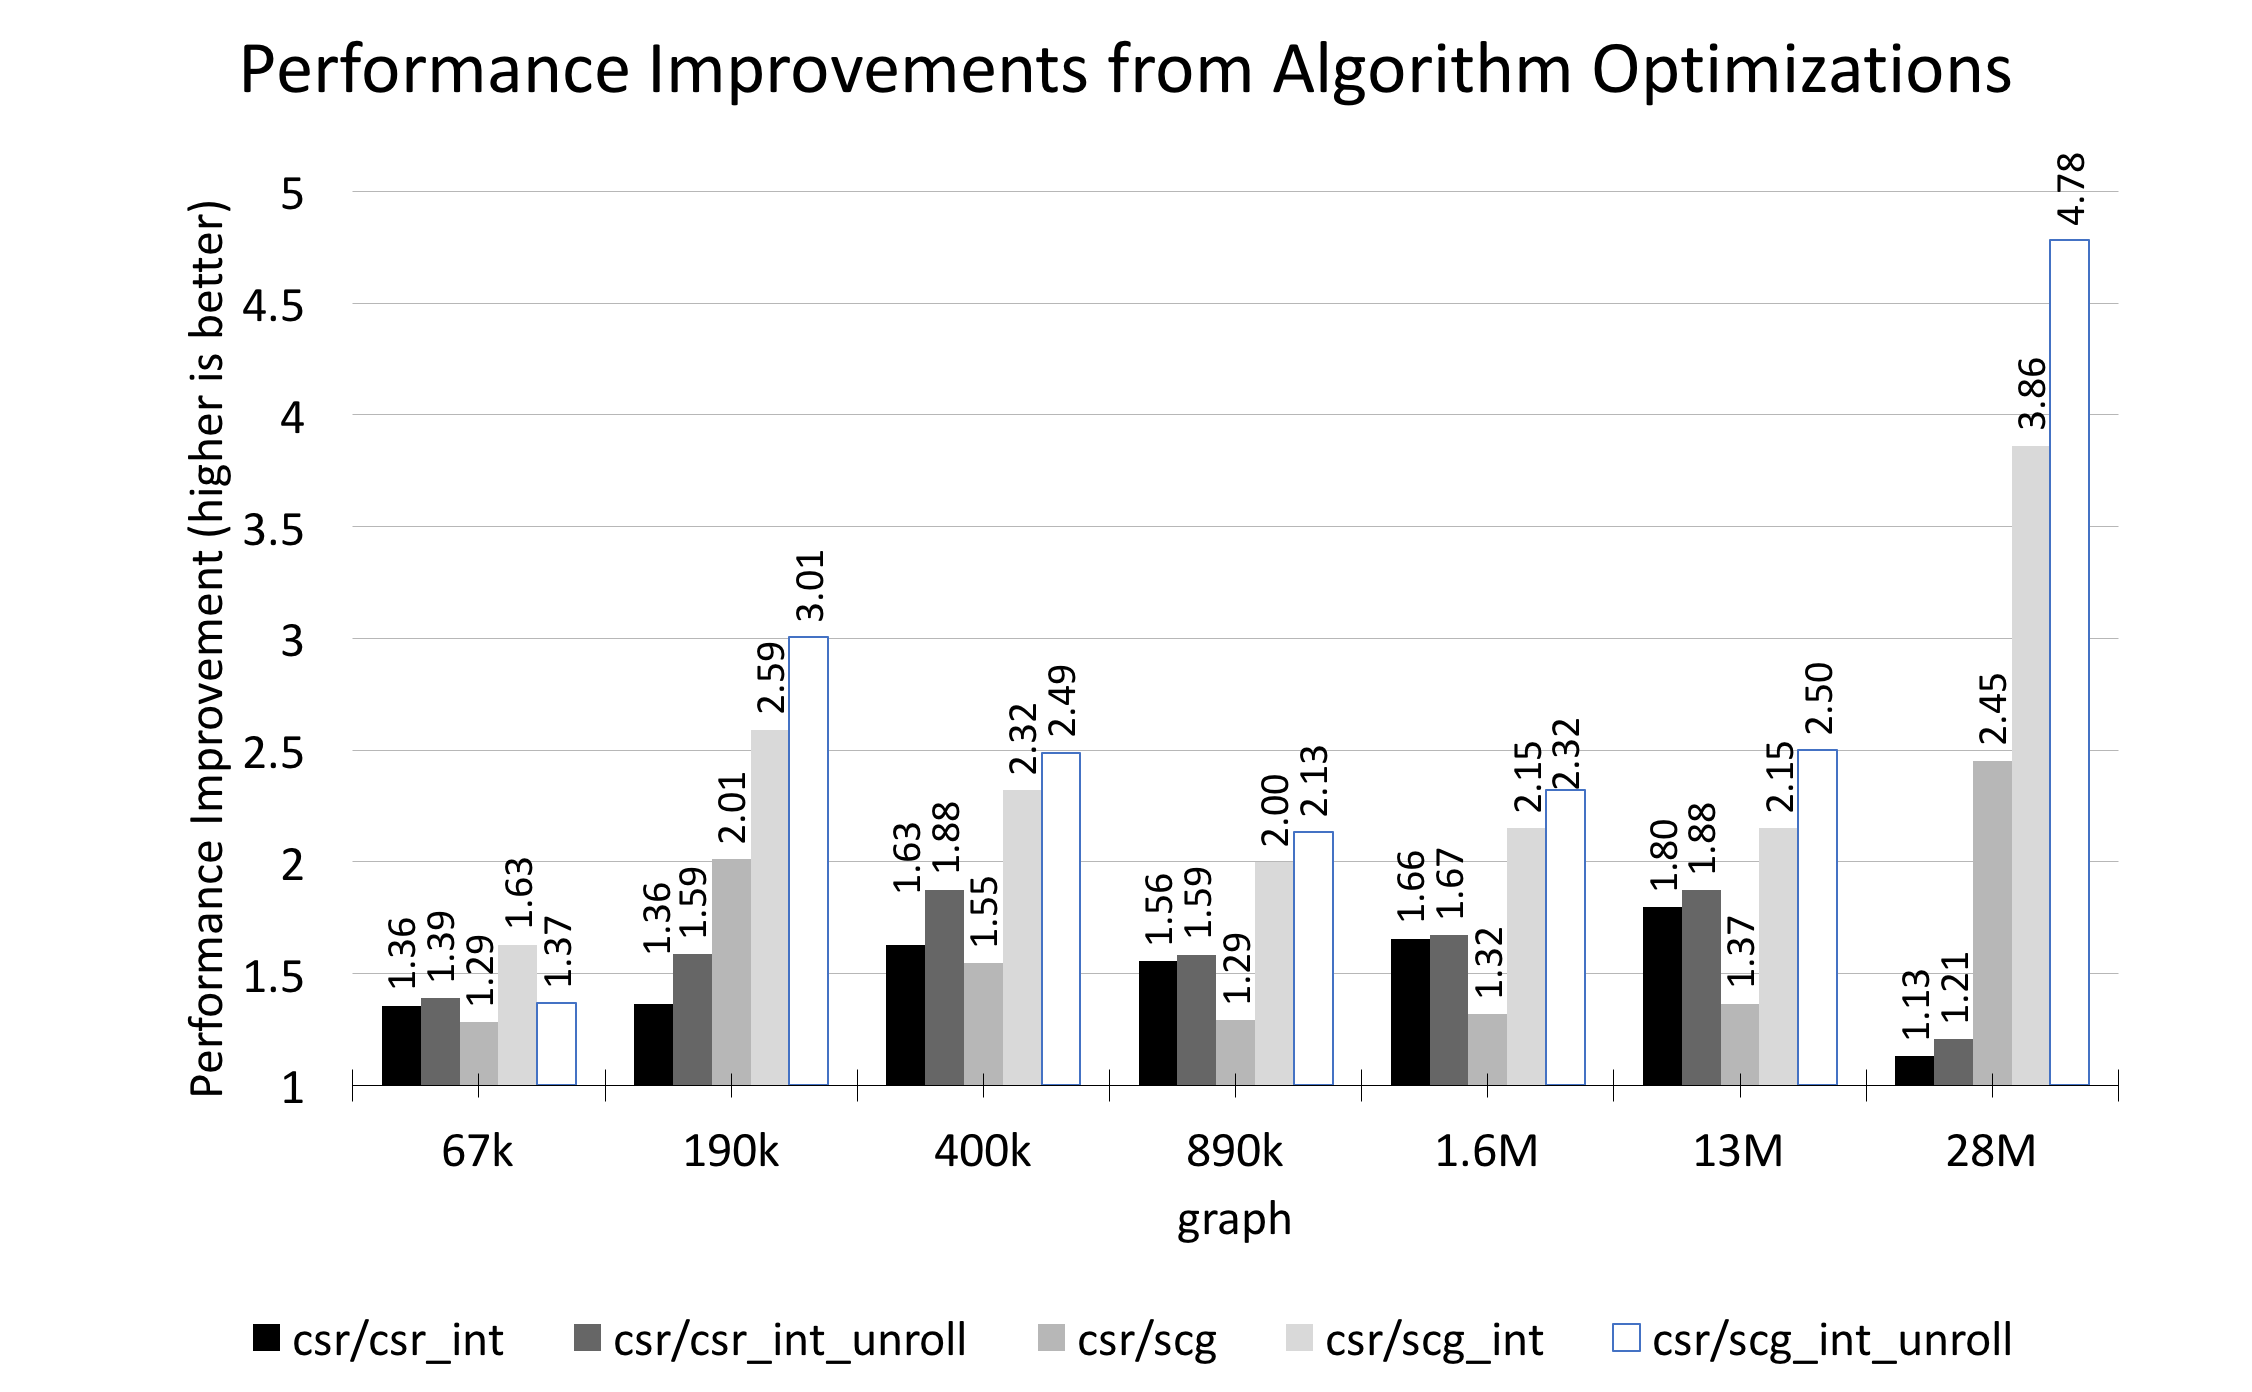
\includegraphics[width=0.8\textwidth]{images/bfsPerformance.png}
  \caption{
    Performance of breadth first traversal implementations.
  }
\end{figure}

On the 28M mesh, the `scg\_int\_unroll' is 11 times
faster than the serial, C++, push implementation, and 4.78 times faster than
the `csr' implementation.
The performance boost given by loop unrolling and use of Sell-C-$\sigma$ are the
result of improved memory coalescing.
Reducing the integer size by half improves performance by 24\% for the 28
million element mesh.

\section{Accelerating Cavity Selection} \label{sec:select}

Accelerating the selection of cavities requires simultaneously evaluating many
cavities.
The current single threaded selection procedure evaluates cavities in order of
their descending distance from the topological center.
Since the ordered selection exposes no concurrency an alternative application of
the topological distance is needed.
The proposed approach applies a parallel topological distance sorting after a
coloring based parallel cavity evaluation has executed.

Critical to concurrent cavity evaluation is avoiding race conditions when
deciding which part to migrate a given graph vertex.
Hyperedge coloring ensures that any two hyperedges that share a common vertex
will be assigned a different color, and thus entire sets of like-colored
hyperedges can be evaluated concurrently.

The Kokkos-kernels graph coloring procedure~\cite{kokkosColoring}
is used to color the hyperedges of the EnGPar hypergraph.
This procedure is driven by a symmetric adjacency matrix.
To color hyperedges we must create the hyperedge-to-vertex-to-hyperedge
graph; the dual of the hypergraph.
The dual graph has one vertex for each hyperedge, and an edge between two
hyperedges if they share at least one common vertex.

The construction of the dual is listed in Algorithm~\ref{alg:dual}.
It starts by making a set, using a Kokkos \texttt{unordered\_map}, that stores
hyperedge-to-hyperedge adjacencies ($l.$\ref{alg:mapStart}-$l.$\ref{alg:mapEnd}).
A parallel reduction and prefix sum then compute the degree list \verb|deg|
($l.$\ref{alg:degStart}-$l.$\ref{alg:degEnd}).
The hyperedge list, \verb|edgeList|, is then filled with a parallel loop over
the hyperedges.
This loop utilizes a Kokkos atomic read-then-increment operation
($l.$\ref{alg:atomic}) to determine the position of the hyperedge in the list of
adjacent hyperedges.
The resulting CSR, \verb|deg| and \verb|edgeList|, are passed directly to
the Kokkos coloring procedure.

\label{alg:dual}
\algloopdefx[PFor]{PFor}[1]{\textbf{parallel for} #1 \textbf{do}}
\algblock[Name]{Start}{End}
\algblockdefx[NAME]{START}{END}
  [1][a]{\textbf{parallel for} #1 \textbf{do}}

\begin{algorithm}
\caption{Dual Graph Converter}
\small
\begin{multicols}{2}
\begin{algorithmic}[1]
\Procedure{dual}{$G=(V,E)$}
  \State $n = 0$ \label{alg:mapStart}
  \PFor{$v \in V$}
    \ForAll{$(i,v) \in E$}
      \ForAll{$(j,v) \in E\setminus\{(i,v)\}$}
        \State $n$++
      \EndFor
    \EndFor 
  \State //n is an upper bound on the set's size
  \State set of int pair $m$ (n)
  \PFor{$v \in V$}
    \ForAll{$(i,v) \in E$}
      \ForAll{$(j,v) \in E\setminus\{(i,v)\}$}
        \State m.
        insert ( $(i,j)$ )
      \EndFor
    \EndFor \label{alg:mapEnd}
  \algstore{convert}
  \end{algorithmic}
  \columnbreak
\begin{algorithmic}[1]
  \algrestore{convert}
  \State $N=|E|$
  \State deg = [$N+1$] \label{alg:degStart}
  \PFor {$k\in m$}
    \State deg($k$.first+1)++
  \PFor{$i=0,1,\ldots,N$}
    \State deg[$i$] = sum(deg[$0:i$]) \label{alg:degEnd}
  \State edgeList = [deg[N]]
  \State degreeCount = [N]
  %\PFor {$k\in m$}
  \START[$k\in m$]
    \State e = deg[k.first] 
    \State i = degreeCount[k.first]++ \label{alg:atomic}
    \State edgeList[e+i] = k.second
  \END
  \EndProcedure
\end{algorithmic}
\end{multicols}
\end{algorithm}

The speedup of the dual and coloring procedures relative to serial
implementations is shown in Figure~\ref{fig:coloringSpeedup}.
Tests were executed on the same system and series of graphs used in
Section~\ref{sec:dist}.
Construction of the dual has a nearly flat speedup relative to the graphs.
Conversely, the speedup of Kokkos coloring improves with graph size.
Profiling of these tests is required to determine how effectively GPU resources
are utilized and identify bottlenecks.

\begin{figure}
  \centering
  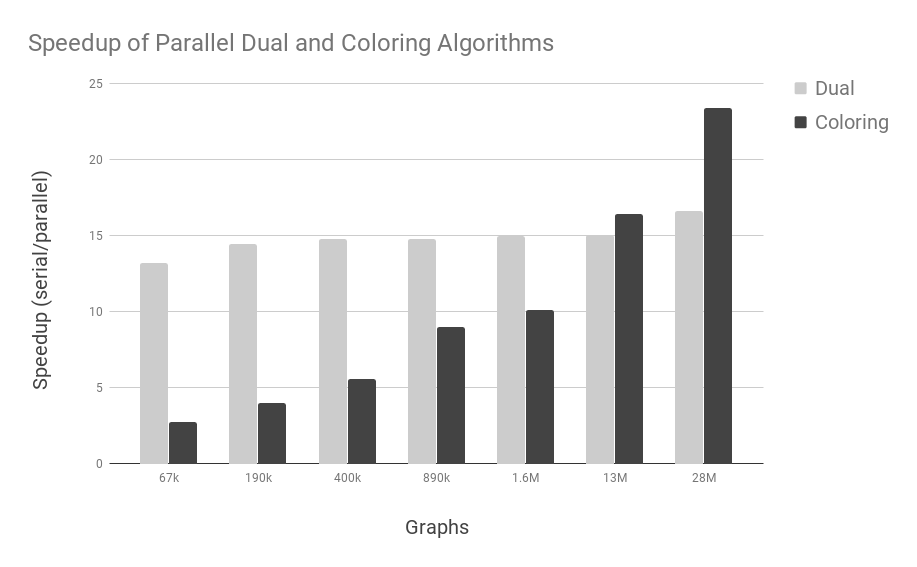
\includegraphics[width=.7\textwidth]{images/Parallel_Speedup.png}
  \caption{The ratio of serial execution time to parallel for dual graph
  construction and graph coloring.}
  \label{fig:coloringSpeedup}
\end{figure}

%\begin{itemize}
%  \item Figure out a better title for this section
%  \item flow control strong scaling case with 1.3B tets: \\
%64Ki \url{https://zenodo.org/record/833519#.WztuxXWYV1M} \\
%128Ki \url{https://zenodo.org/record/834946#.Wztu-HWYV1M} \\
%256Ki \url{https://zenodo.org/record/835483#.WztvCXWYV1M} \\
%512Ki \url{https://zenodo.org/record/835742#.WztvG3WYV1M}
%  \item the number of elements per-process may be too small for nodes with large GPUs to run efficiently (data transfer may become more costly than running the selection on the CPU!) - especially as we approach 512Ki parts
%  \item we will have to run the condense tool to create an 2Ki (640k elms/part),
%    4Ki (320k), 8Ki (160k), 16Ki (80k), and 32Ki (40k) meshes -
%    fun3d uses between 75M and 2.3M elements per GPU on summitdev (from siampp18
%    presentation)
%  \item run on ORNL titan or summit (if accessible)
%  \item compare runtimes versus results from SC17 paper~\cite{engparSC17}
%  \item use mesh vertex = graph vertex and mesh edge = graph edge for tests -
%    will need to run MPI only engpar to establish the baseline performance
%  \item plot the time spent in MPI only selection vs kokkos coloring selection
%    vs part size - the comparison must start and end at equivalent points in the
%    code - start before selection and end just before migration (or whatever the
%    next stage) begins
%  \item plot the breakdown of time spent in coloring selection vs part size -
%    data transfer, color computation, selection (possibly broken into cavity
%    selection and filtering for distance), tranferring the selection list
%    back to the host
%  \item I expect there will be some reduction in partition quality using the
%    coloring based selection since we won't have as fine-grained control over
%    the process as the MPI only procedure.  As long as the quality reduction is
%    controlled and performance is better we should be OK.
%\end{itemize}

\section{Closing Remarks} \label{sec:closing}
Speedup results of two critical procedures used by EnGPar were demonstrated.
Parallel distance computation performance is over an order of magnitude greater
and is a direct replacement for the existing procedure.
Parallel coloring for the selection process demonstrates high performance
across a range of mesh sizes.
Ongoing work is focused on fully integrating these advances into the production
version for evaluation of overall performance and partition quality.

\begin{acknowledgement}
This research was supported by the U.S. Department of Energy, Office of Science,
Office of Advanced Scientific Computing Research, under award DE-SC00066117
(FASTMath SciDAC Institute) and by the National Science Foundation under Grant
No. ACI 1533581, (SI2-SSE: Fast Dynamic Load Balancing Tools for Extreme Scale
Systems).
Any opinions, findings, and conclusions or recommendations expressed in this
material are those of the author(s) and do not necessarily reflect the views
of the National Science Foundation.
\end{acknowledgement}

\bibliographystyle{acm}
\bibliography{scorec-refs/scorec-refs}
\end{document}
